\chapter{Einleitung}
Im letzten Jahr habe ich mich damit beschäftigt, wie man mithilfe eines Raspberry Pi Umweltdaten messen, aufzeichnen und auswerten kann. Hierzu verwende ich mehrere Sensoren, die die Lufttemperatur (sowohl im Klassenraum, als auch außen), Luftfeuchtigkeit, Luftdruck und die relative Luftqualität. Diese Daten werden als \gls{CSV} gespeichert und können grafisch und rechnerisch ausgewertet werden. 

Die grafische Auswertung läuft über ein Webinterface, das innerhalb der Schule aufrufbar ist. Von außerhalb ist eine regelmäßig aktualisierte Kopie unter \href{http://winkler.kremszeile.at/}{winkler.kremszeile.at} erreichbar. Auf dieser Seite können neben allgemeinen Informationen über das Projekt und Links zu weiteren Informationen\footnote{siehe Anhang \ref{anhang:weitere_informationen}} die aktuellen Messwerte als Balken-Diagramm, welches sich selbst aktualisiert, und die komplette Aufzeichnung als interaktives Diagramm dargestellt werden.

Unabhängig davon können mit einem von mir geschriebenen \gls{Python}-Programm die Daten einer Messung im Nachhinein mathematisch ausgewertet werden.

Um diese Vorwissenschaftliche Arbeit so verständlich wie möglich zu halten, werden Wörter, die im Text farbig hervorgehoben sind, im Glossar auf Seite \pageref{main} erklärt.

\begin{figure}[h]
  \centering
     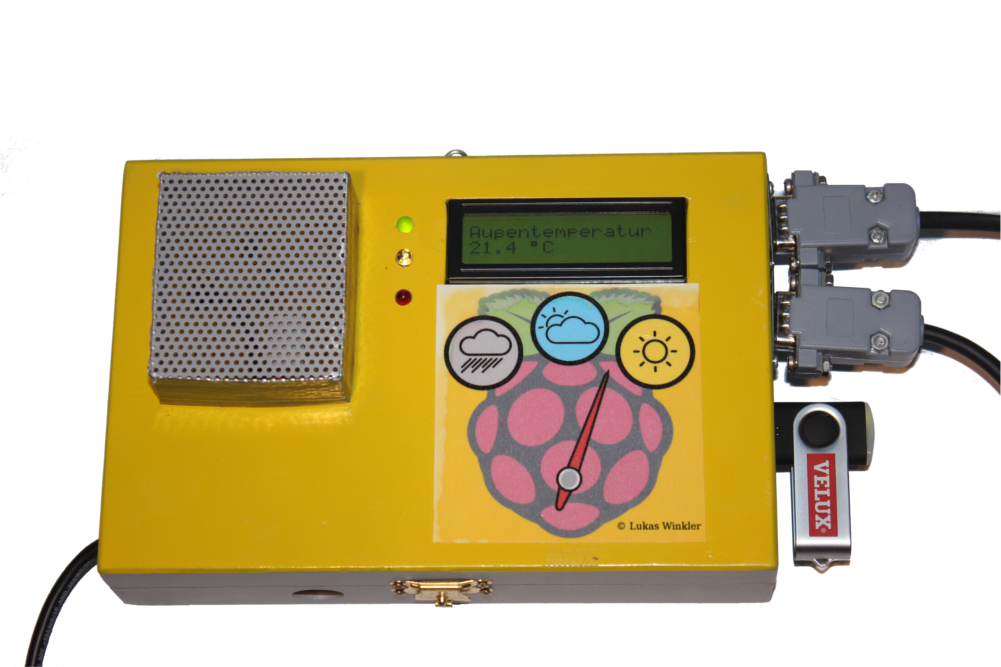
\includegraphics[width=\textwidth]{figures/gesamt.png}
  \caption{Messstation}
  \label{fig:gesamt}
\end{figure}